

\textbf{Limitation}

There is an important difference between the human leg and most robotic setups in which the typical joint angle algorithms are employed: It is very difficult to attach IMUs to the leg in such a way that one of the local coordinate axes aligns exactly with the knee joint axis \cite{seel_imu-based_2014}. 

A problem in IMU-based human motion analysis is that the IMU's local coordinate axes are not aligned with any physiologically meaningful axis.



\subsubsection{Mahony filter}

The Mahony filter proposed by Rober Mahony and collegues \cite{mahony_nonlinear_2008}, is a quaternion based sensor fusion algorithm designed for attitude estimation. It is a nonlinear complementary filter for three dimensional rotation, especially designed to leverage gyroscope and accelerometer data obtained from typical low cost IMUs, chractarized by high noise levvels and time varying additive biases, to estimate orientation in real-time. This makes it a very viable choise for computing the orientations of the thigh and shank IMUs.


\textit{Theoretical Implementation}
The mahony filter is 






\textit{Madgwick Filter}


The orientation of the IMU can be represented by a quaternion, a rotation matrix or Euler angles. 

subsection{Kalman Filter for Knee Angle Estimation}

The Kalman filter is a widely recognized state-space algorithm that utilizes a probabilistic framework for sensor fusion. Its ability to optimally combine noisy sensor measurements with a mathematical model of the system makes it a robust choice for orientation and angle estimation tasks. For knee angle estimation, the Kalman filter could integrate data from IMUs mounted on the thigh and shank, combining gyroscope data for angular velocity and accelerometer data for long-term stability. The application of the Kalman filter in this context involves estimating the relative orientation of the two IMUs and, subsequently, the knee joint angle.

### Filter Framework

The Kalman filter operates in two primary stages: prediction and correction. In the prediction stage, the state vector \( \mathbf{x}_k \), which could include orientation, angular velocity, and drift, is estimated based on the system dynamics:

\[
\mathbf{x}_{k|k-1} = \mathbf{A} \mathbf{x}_{k-1} + \mathbf{B} \mathbf{u}_{k-1}
\]

where:
- \( \mathbf{x}_{k|k-1} \) is the predicted state vector,
- \( \mathbf{A} \) is the state transition matrix that models the dynamics of the system, such as the motion of the thigh and shank,
- \( \mathbf{B} \) relates the control inputs (e.g., gyroscope angular velocity \( \mathbf{u}_{k-1} \)) to the system.

In the correction stage, the predicted state is updated using measurements from the IMUs, such as accelerometer readings that provide a gravity reference:

\[
\mathbf{x}_{k|k} = \mathbf{x}_{k|k-1} + \mathbf{K}_k \left( \mathbf{z}_k - \mathbf{H} \mathbf{x}_{k|k-1} \right)
\]

Here:
- \( \mathbf{z}_k \) is the measurement vector from sensors,
- \( \mathbf{H} \) maps the state vector to the measurement space,
- \( \mathbf{K}_k \), the Kalman gain, determines the weight given to the sensor measurements relative to the prediction.

### Potential Benefits for Knee Angle Estimation

The Kalman filter is theoretically well-suited for estimating knee angles as it can model both the orientation dynamics and the measurement uncertainties. The ability to incorporate multiple sources of information, such as gyroscope, accelerometer, and magnetometer data, makes it robust against individual sensor limitations. For example:
- Gyroscope data provides high-resolution angular velocity information but suffers from drift over time.
- Accelerometer data provides long-term stability by detecting the direction of gravity but is susceptible to high-frequency noise and motion artifacts.

The Kalman filter combines these data sources to produce an optimal estimate of the IMUs' relative orientation, which can then be used to compute the knee angle.

### Challenges in Real-Time Knee Angle Estimation

Despite its strengths, the Kalman filter presents significant challenges when applied to real-time knee angle estimation during gait. First, the filter requires a well-defined state-space model, including the state transition matrix \( \mathbf{A} \) and observation matrix \( \mathbf{H} \). Defining these matrices for human gait dynamics is inherently complex due to the non-linear and variable nature of human motion.

Second, the computational complexity of the Kalman filter is non-trivial. Each iteration involves matrix multiplications and inversions, which can become computationally expensive, especially in systems with limited processing power. This could introduce latency in real-time applications, degrading the responsiveness of the feedback loop in functional electrical stimulation (FES) systems.

Finally, the performance of the Kalman filter heavily depends on the correct tuning of the process noise covariance matrix \( \mathbf{Q} \) and the measurement noise covariance matrix \( \mathbf{R} \). These parameters influence the balance between the predicted state and sensor measurements. Improper tuning can result in either overly conservative estimates (ignoring valid measurements) or excessive reliance on noisy data.

### Evaluation for Knee Angle Estimation

For knee angle estimation in a real-time FES system, the Kalman filter provides high theoretical accuracy but at the cost of complexity and computational demand. The challenges in accurately modeling human gait dynamics, combined with the processing overhead, make the Kalman filter less practical for systems requiring low-latency feedback. Simpler algorithms, such as the Madgwick filter, which do not rely on predefined models and have lower computational requirements, are often preferred in this application.

Nonetheless, the Kalman filter could be advantageous in scenarios where high computational resources are available, or in research environments where precision is prioritized over real-time performance. For readers seeking a comprehensive introduction to the Kalman filter, including its derivation and practical applications, the text \textit{"Kalman Filtering: Theory and Practice with MATLAB"} by Grewal and Andrews provides a detailed and reliable reference \cite{grewal_kalman_2015}.















### Extended Kalman Filter for Orientation Estimation in Knee Angle Calculation

The Extended Kalman Filter (EKF) is a widely used algorithm for state estimation in non-linear systems. Its adaptability to non-linear dynamics and observations makes it a robust choice for orientation estimation using data from IMUs. When applied to knee angle estimation, the EKF provides a framework to combine gyroscope and accelerometer data to derive the relative orientation of the thigh and shank, which can be used to compute the knee angle in real time.

#### Theoretical Foundation of the EKF

The EKF extends the Kalman filter to handle non-linear system dynamics and observation models by linearizing these functions around the current state estimate. In this context, the state vector represents the orientation of the IMU, typically expressed as a quaternion:
\[
\mathbf{x} = 
\begin{bmatrix}
q_w & q_x & q_y & q_z
\end{bmatrix}^T
\]
where \( q_w, q_x, q_y, q_z \) are the components of the quaternion describing the rotation of the IMU with respect to a reference frame. The filter uses a process model to predict the next state and a measurement model to correct the prediction using sensor data.

#### Prediction Step

The prediction step estimates the next orientation based on angular velocity measurements from the gyroscope. The non-linear quaternion dynamics are given by:
\[
\dot{\mathbf{q}} = \frac{1}{2} \mathbf{q} \otimes \mathbf{\omega}
\]
where \( \mathbf{\omega} \) is the angular velocity vector measured by the gyroscope, and \( \otimes \) denotes quaternion multiplication. For discrete time steps, the quaternion update can be approximated as:
\[
\mathbf{q}_{k|k-1} = \mathbf{q}_{k-1} + \frac{\Delta t}{2} \mathbf{q}_{k-1} \otimes \mathbf{\omega}_k
\]
where \( \Delta t \) is the sampling interval.

The state covariance matrix is updated during the prediction step to account for process noise:
\[
\mathbf{P}_{k|k-1} = \mathbf{F}_k \mathbf{P}_{k-1} \mathbf{F}_k^T + \mathbf{Q}_k
\]
where \( \mathbf{F}_k \) is the Jacobian of the process model with respect to the state, and \( \mathbf{Q}_k \) is the process noise covariance matrix, derived from gyroscope noise characteristics.

#### Correction Step

The correction step integrates accelerometer data to refine the orientation estimate. The accelerometer provides a measurement of the gravity vector in the sensor frame, which can be compared to the predicted gravity vector derived from the estimated orientation. The measurement model is given by:
\[
\mathbf{z}_k = h(\mathbf{q}_k) = \mathbf{R}(\mathbf{q}_k) \mathbf{g}
\]
where \( \mathbf{R}(\mathbf{q}_k) \) is the rotation matrix corresponding to the predicted quaternion \( \mathbf{q}_k \), and \( \mathbf{g} \) is the gravity vector in the global frame.

The innovation, or measurement residual, is computed as:
\[
\mathbf{y}_k = \mathbf{z}_k^{\text{meas}} - h(\mathbf{q}_{k|k-1})
\]
The Kalman gain, which determines the weight given to the innovation, is calculated as:
\[
\mathbf{K}_k = \mathbf{P}_{k|k-1} \mathbf{H}_k^T (\mathbf{H}_k \mathbf{P}_{k|k-1} \mathbf{H}_k^T + \mathbf{R}_k)^{-1}
\]
where \( \mathbf{H}_k \) is the Jacobian of the measurement model, and \( \mathbf{R}_k \) is the measurement noise covariance matrix derived from accelerometer noise characteristics.

The corrected state is updated as:
\[
\mathbf{q}_{k|k} = \mathbf{q}_{k|k-1} + \mathbf{K}_k \mathbf{y}_k
\]
To ensure the quaternion remains a unit quaternion, it is normalized after each update.

#### Evaluation for Real-Time Knee Angle Estimation

The EKF is well-suited for orientation estimation due to its ability to handle the non-linear dynamics of quaternion-based rotations. By combining gyroscope data for short-term angular velocity tracking with accelerometer data for long-term stability, the EKF provides robust orientation estimates that can be used to calculate the knee angle as the relative orientation between the thigh and shank IMUs.

However, there are challenges associated with using the EKF for real-time knee angle estimation:
1. **Computational Complexity**: The EKF requires the computation of Jacobians and matrix multiplications, which can introduce latency in resource-constrained systems. For real-time applications, these computational demands must be carefully managed.
2. **Sensitivity to Noise**: While the EKF effectively handles Gaussian noise, it relies on accurate noise covariance matrices (\( \mathbf{Q}_k \) and \( \mathbf{R}_k \)) for optimal performance. Poorly tuned covariance matrices can degrade the accuracy of the filter.
3. **Initialization and Drift**: The EKF requires an accurate initial orientation estimate to avoid divergence. Additionally, any uncorrected bias in the gyroscope data can lead to drift in the orientation estimates over time.

Despite these challenges, the EKF provides a strong balance between accuracy and adaptability, making it a viable choice for knee angle estimation. When magnetometer data is unavailable, as in this case, the filter can still perform effectively by leveraging the complementary strengths of gyroscope and accelerometer data. For systems with limited processing power, however, alternative algorithms such as the Madgwick filter may offer a more computationally efficient solution.

The EKF’s ability to integrate sensor data in a probabilistic framework ensures that it remains a cornerstone of orientation estimation techniques, particularly in applications requiring dynamic motion tracking. Properly implemented and tuned, it is capable of providing reliable orientation estimates critical for computing knee angles in real-time functional electrical stimulation systems.





\subsubsection{Simplified Curve}
The first mathematical representation of the
The resulting curve modeled as the sum of two sinusoidal components, defined as:
\[
y(x) =
\begin{cases}
A_1 \sin\left(2 \pi f_1 x + \phi_1\right) + C_1, & 0 \leq x \leq 40 \\
A_2 \sin\left(2 \pi f_2 x + \phi_2\right) + C_2, & x > 40
\end{cases}
\]
where the parameters are defined as:

For the first bump:
\[
A_1 = 11, \quad f_1 = \frac{0.1}{4}, \quad \phi_1 = \frac{\pi}{2} + 2\pi f_1 \cdot 20, \quad C_1 = 15
\]

For the second bump:
\[
A_2 = 30, \quad f_2 = \frac{0.1}{6}, \quad \phi_2 = -\frac{\pi}{2} + 2\pi f_2 \cdot 80, \quad C_2 = 34
\]


A visualization of this curve can be seen in figure \ref{fig:simplecurve}. When comparing this however with the typical knee angle curve there are some major differences such as the height of the end of the second sinus curbe and height of the valley between the two curves. Because of these discrepancies another approach was attempted.
\begin{figure} [h]
    \centering
    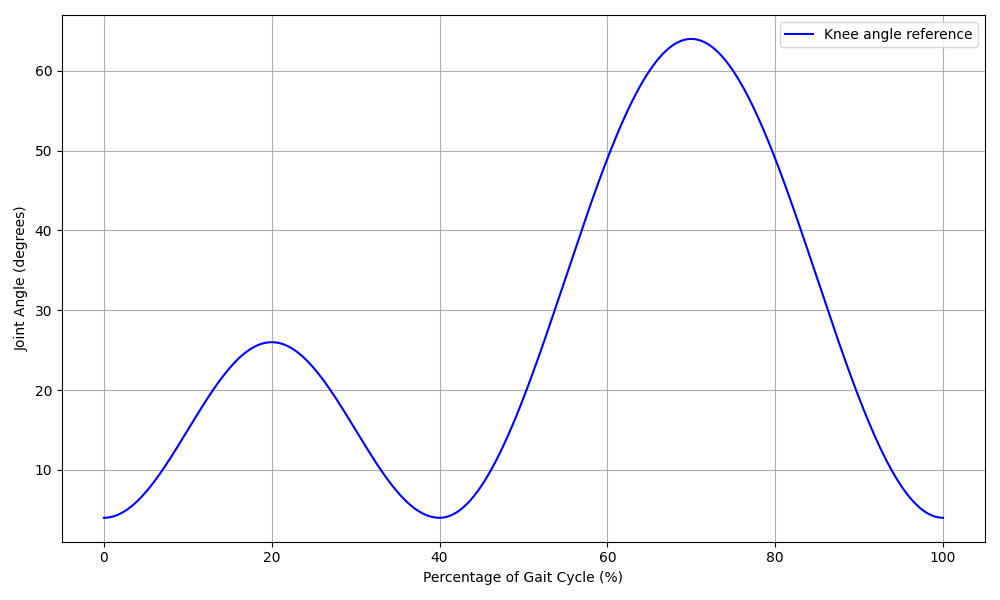
\includegraphics[width=0.8\linewidth]{images/simpleKneeAngle.png}
    \caption{Simplified knee angle curve during gait, created by combining two sinusoids}
    \label{fig:simplecurve}
\end{figure}
